\chapter{Search for invisibly decaying VBF produced Higgs bosons in Run 1 prompt data}
\label{chap:prompt}
%Introduction to selection and challenges of jets+met, e.g. trigger, QCD
As described in \ChapterRef{chap:theory}, searches for invisible Higgs boson decays are well motivated by their sensitivity to new physics, such as \ac{DM}. Because the invisible branching of an \ac{SM} 125 \GeV\, Higgs boson is very small, any observation made of invisible Higgs boson decays at the \LHC would be evidence for physics beyond the \ac{SM}. This chapter describes the search for invisible Higgs boson decays using data taken by CMS in 2012 with a promptly reconstructed trigger developed specifically for this analysis. The total integrated luminosity collected with this trigger that was certified for use in physics analyses was 19.5\invfb~. The analysis was published in \ReferenceRef{Chatrchyan:2014tja}.

\section{Event selection}
\label{sec:promptsel}
%describe backgrounds and motivate selection
In signal events it is expected that there will be two jets with a characteristic \ac{VBF} topology and a large amount of \MET. Several background processes, with significantly higher cross-sections than the signal process, can also produce events with these objects present. It is therefore necessary to design selection criteria, known as ``cuts'', to remove as many of these background events from the analysis as possible.

The most significant of these background processes is the production of a vector boson in association with jets. Leptonic decays of \PW bosons and \PZ boson decays to neutrinos both produce \MET and, due to the approximately 1000 times higher cross-section for vector boson production than Higgs boson production, there are many events where the associated jets have a \ac{VBF}-like topology, collectively these backgrounds are referred to as ``$V$+jets''. %??relative cross-section
A further background process that can produce significant numbers of \ac{VBF}-like jets due to its very large cross-section is QCD production of multiple jets (``QCD multijets''). Whilst these multijet events have very little \MET from real invisible particles, it is possible for significant ``fake'' \MET to be caused by mismeasurement of the jets. The production of two vector bosons or top quarks can also lead to two jets and real \MET, although they have much lower cross-sections than the other background processes and their contribution is not as significant.

%trigger requirements and design
\subsection{Trigger}
\label{sec:prompttrig}
The trigger requirements can be viewed as the first stage of the event selection. Their primary role is to reduce the rate of events that must be recorded by the detector whilst retaining the maximum number of signal events. As described in \SectionRef{sec:triggers} the decision whether to keep an event must be made very rapidly, and as a result the object reconstruction algorithms used are less sophisticated, and the available detector resolution is worse, than those offline. The trigger criteria have therefore been chosen to be as loose as possible whilst maintaining the required rate reduction.

To pass the \ac{L1} trigger selection events are required to have \MET$>40$ \GeV. Events are then required to have \METnoMU$>65$\GeV\, and that at least one pair of jets in the event is \ac{VBF}-like to pass the \ac{HLT} selection. The \ac{VBF}-like requirements on the jets consist of requiring their $\eta$ separation, $\Delta\eta_{jj}$, be greater than 3.5, that they are in opposite forward/backward halves of the detector and that they have high invariant mass, $M_{jj}>800 \GeV$. The use of \METnoMU at trigger level ensures that events which are needed for the control regions used in the background estimation techniques described in \SectionRef{sec:promptbkg} are not rejected. Not requiring that the \ac{VBF}-like pair of jets also be the two highest \pt jets reduces inefficiencies caused by different \pt orderings in jets reconstructed by the trigger and by the offline reconstruction. The efficiency for events to pass the trigger as a function of their values of several offline variables is shown in \FigureRef{fig:prompttrigplots}. The measured trigger efficiency is applied as a weight to all \ac{MC} samples.

%trigger efficiency plots
\begin{figure}
  \subfloat[]{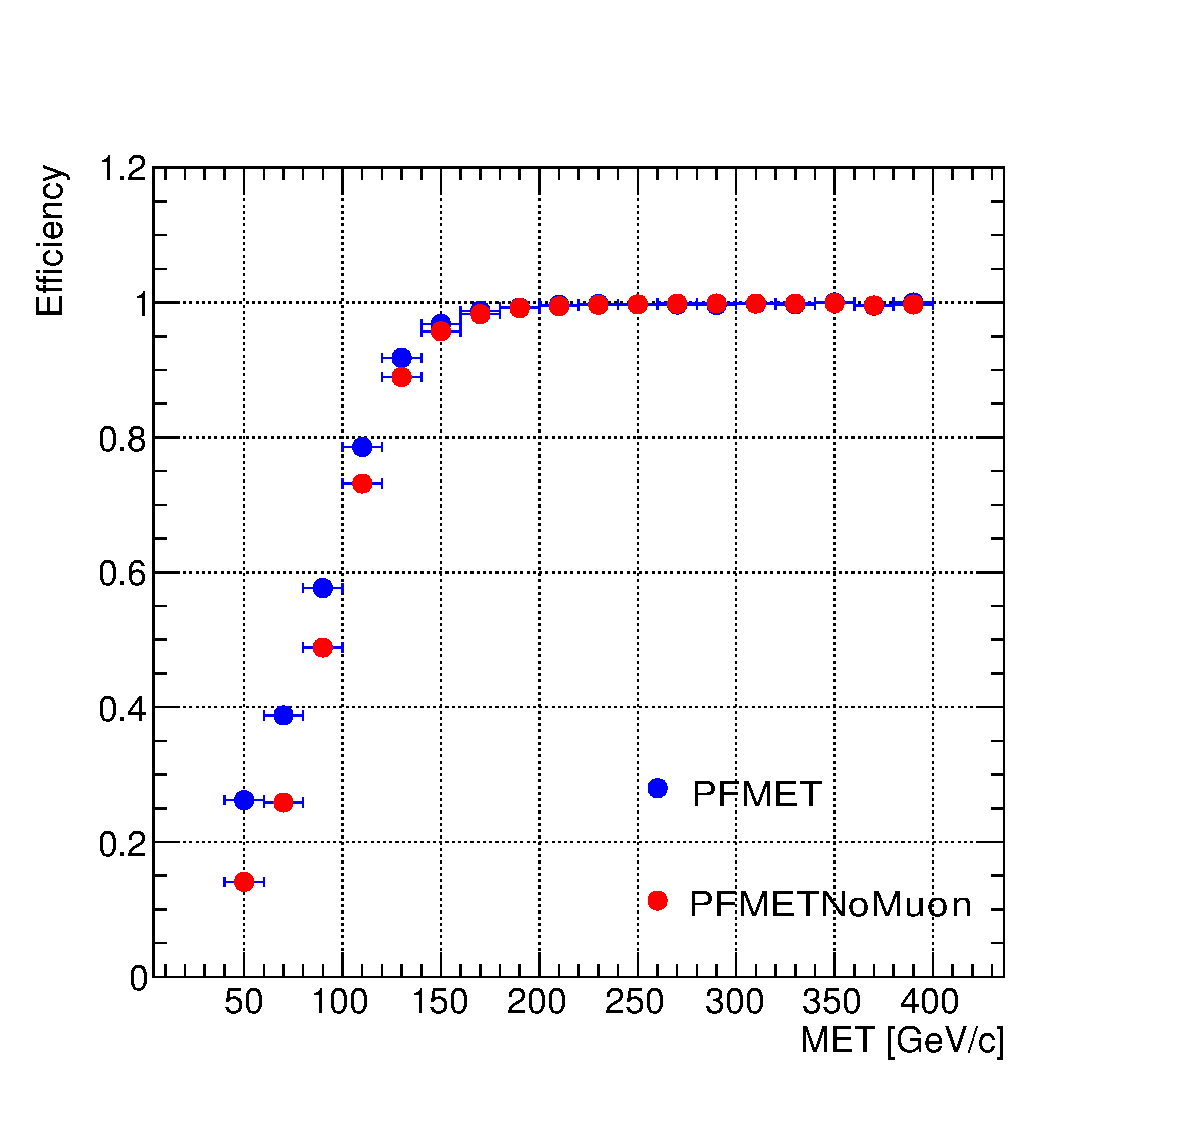
\includegraphics[width=.6\largefigwidth]{plots/prompt/TrigEff_SingleMu_L1ETM40.pdf}}
  \subfloat[]{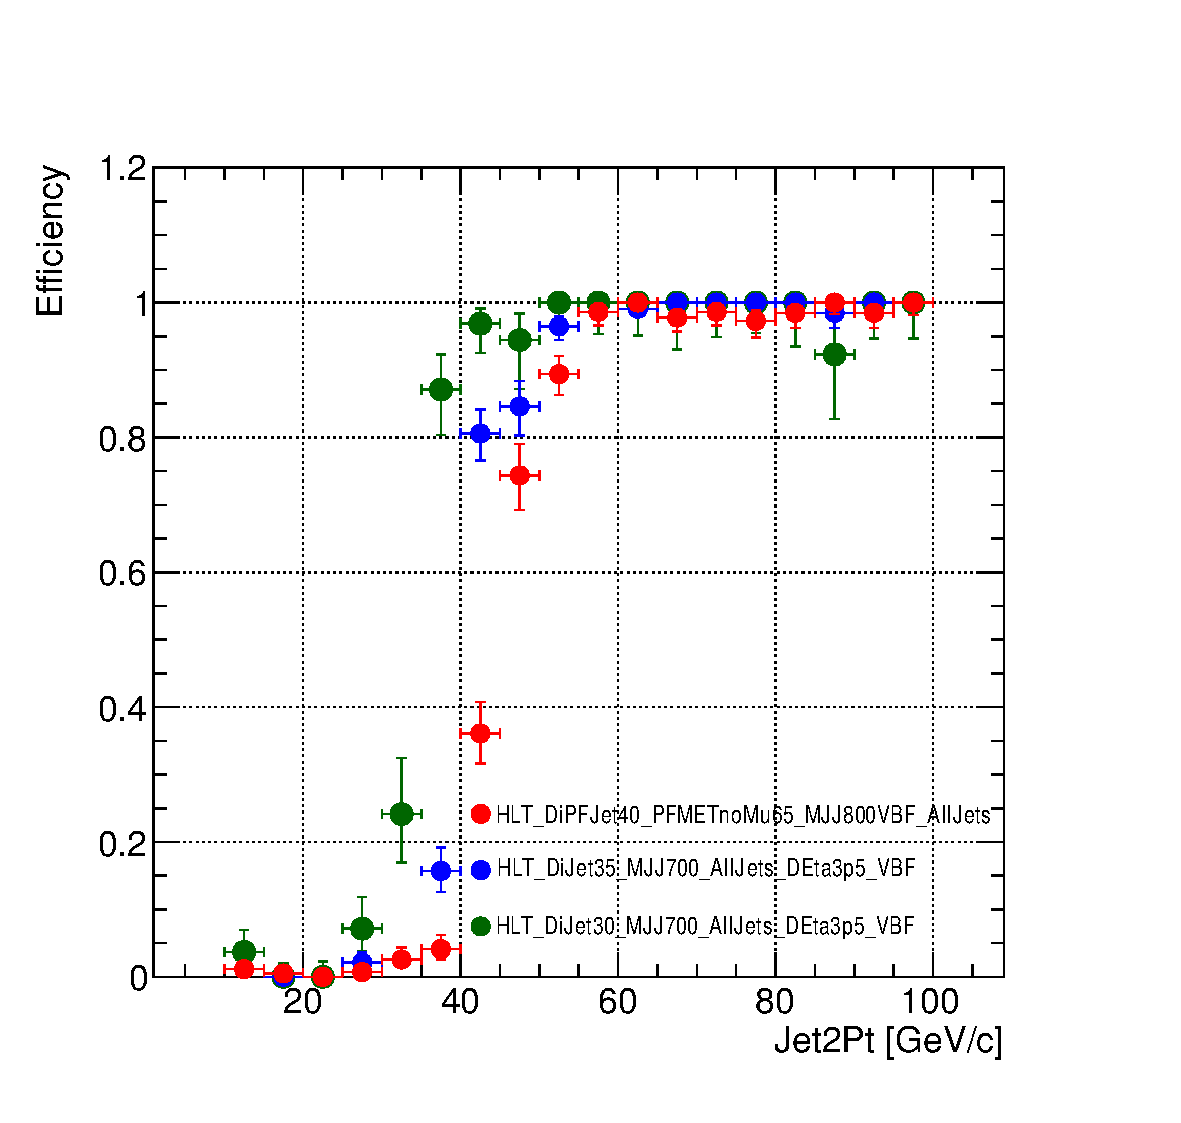
\includegraphics[width=.6\largefigwidth]{plots/prompt/TrigEff_SingleMu_Jet2Pt.pdf}}

  \subfloat[]{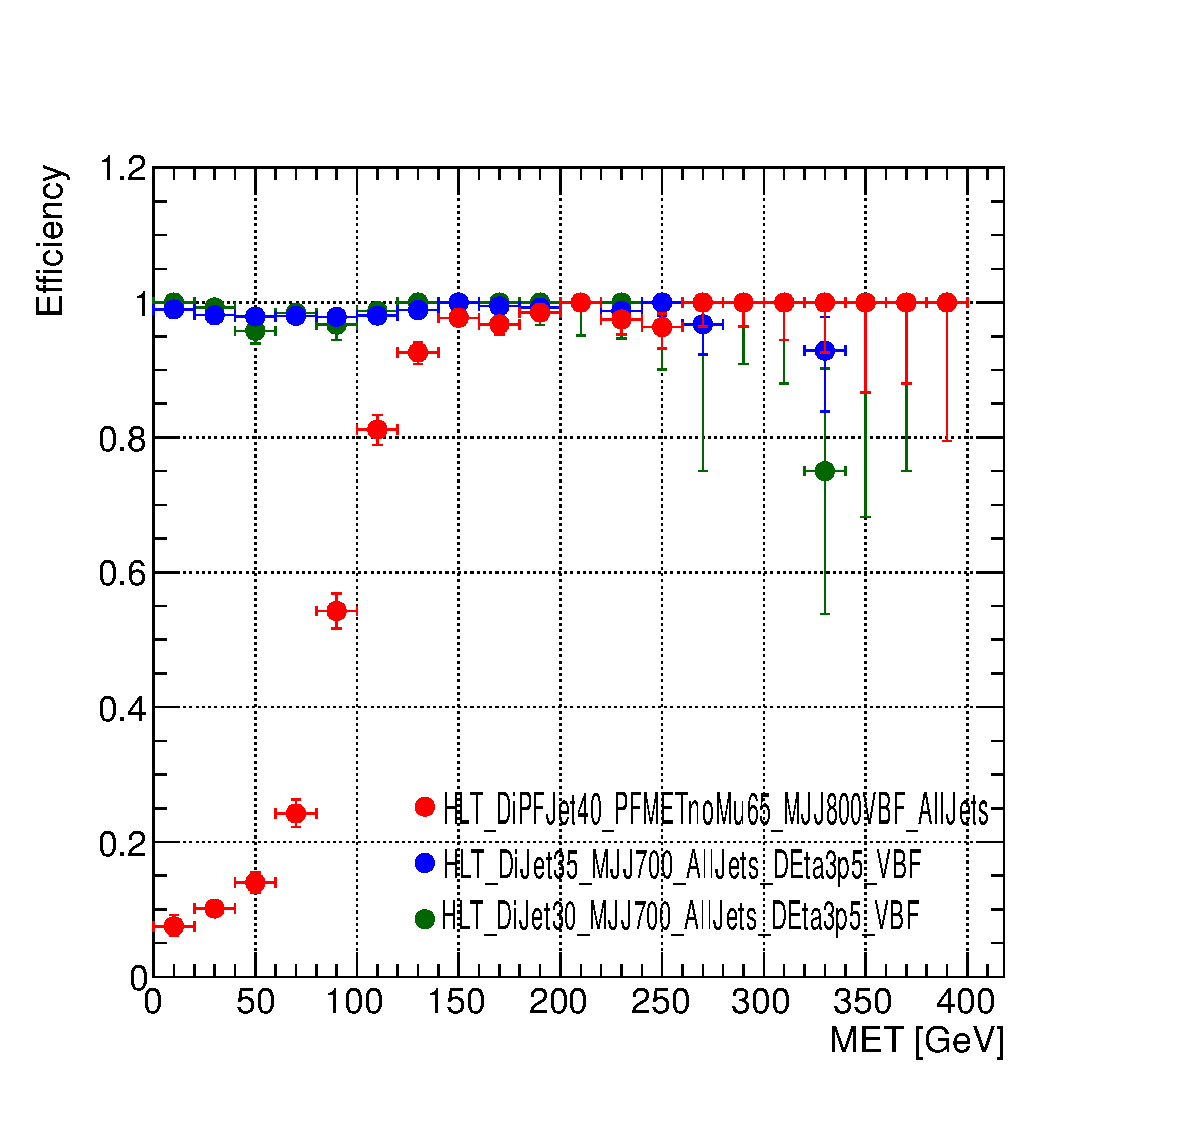
\includegraphics[width=.6\largefigwidth]{plots/prompt/TrigEff_SingleMu_MET.pdf}}
  \subfloat[]{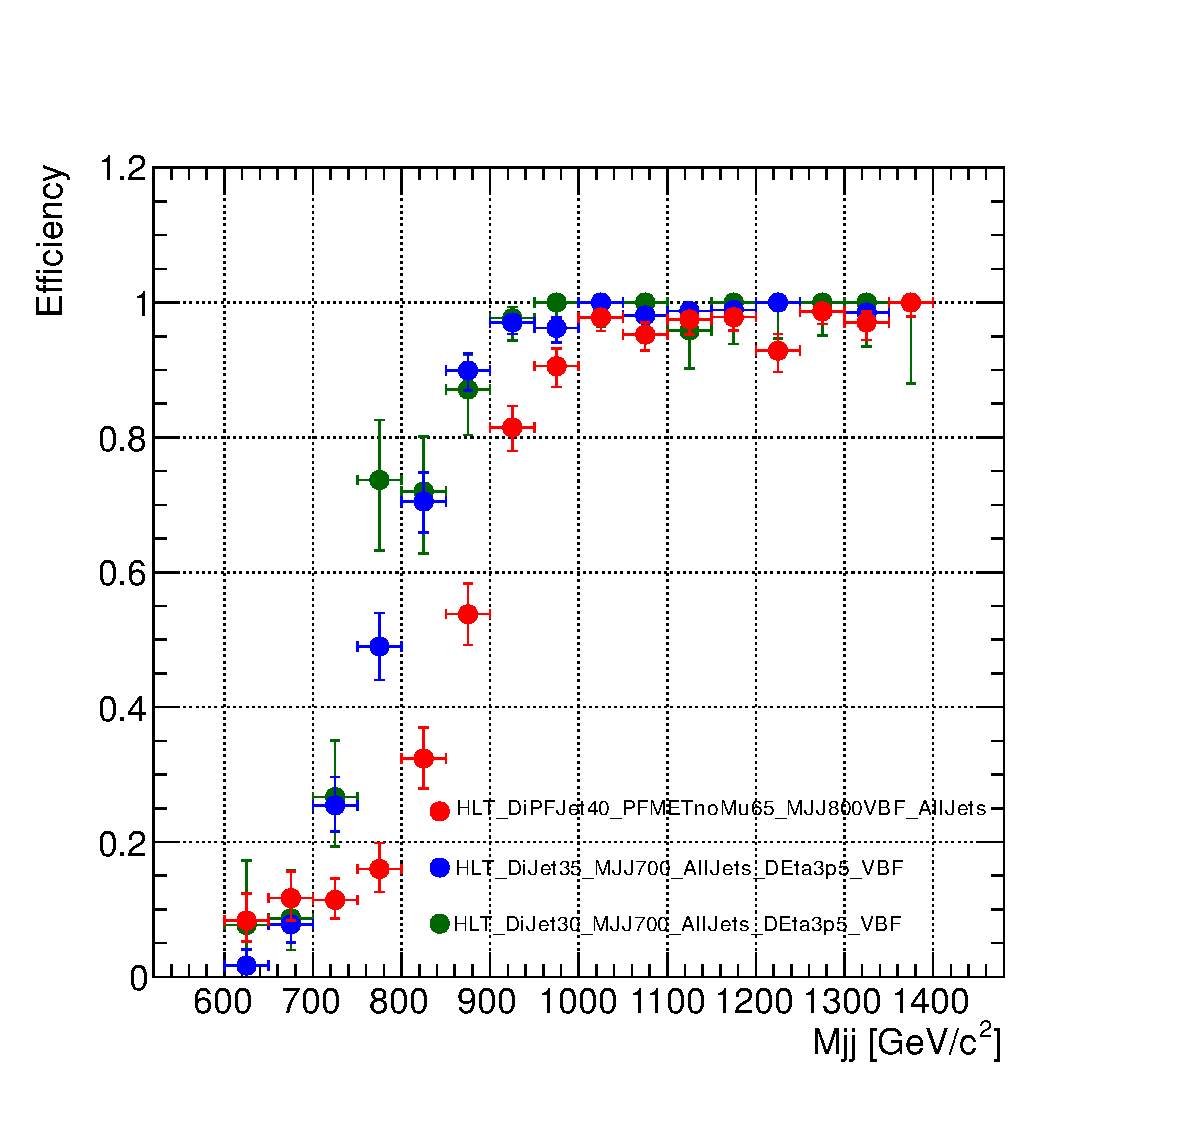
\includegraphics[width=.6\largefigwidth]{plots/prompt/TrigEff_SingleMu_Mjj.pdf}}
  \caption{The trigger efficiency as a function of the values of several offline variables, measured in a sample of events recorded on a single-muon trigger. (a) \ac{L1} trigger efficiency as a function of offline \MET and \METnoMU, (b) \ac{HLT} efficiency as a function of second highest offline jet \pt, (c) \ac{HLT} efficiency as a function of offline \MET, (d) \ac{HLT} efficiency as a function of $M_{jj}$~\cite{ARTICLE:CMSAN-12-403} .}
  \label{fig:prompttrigplots}
\end{figure}

\subsection{Offline selection}
\label{sec:promptofflinesel}
%selection and motivation
The offline selection begins by requiring that events have no veto muons or electrons, as defined in sections \ref{sec:electrons} and \ref{sec:muons}, with \pt$>10$ \GeV. This lepton veto reduces the background from \PW and \PZ boson decays and also from top quarks. The two highest \pt jets in the event are then identified as the VBF tag pair. Tighter versions of the trigger selection are then applied. The tag jets are required to be in opposite forward/backward halves of the detector, to both have \pt$>50$ \GeV\, and $|\eta|<4.7$, to have $M_{jj}>1100$ \GeV and $\Delta\eta_{jj}>4.2$. The \METnoMU is required to be greater than 130 \GeV. Because events with veto muons have been vetoed \METnoMU is in the case of the signal region identical to \MET. However, it is important for background estimation methods that \METnoMU and not \MET is used.

As well as the trigger based selection further cuts are made to reduce the QCD multijet background to a level much lower than the V+jets backgrounds. The two tag jets are required to have an azimuthal separation, $\Delta\phi_{jj}<1.0$, since multijet events with \MET due to mismeasurement are most likely to have their jets back-to-back in the detector, i.e. with $\Delta\phi_{jj}=\pi$. Events where there are any jets with \pt$>30$ \GeV\, between the two tag jets in $\eta$ are also vetoed. This \ac{CJV} is motivated by the lack of colour connection, described in \SectionRef{sec:higprod}, between the quarks in VBF production that makes the presence of such jets unlikely in genuine signal events.

The specific values of the cuts on each variable are chosen for three reasons. Firstly, the reconstruction algorithms for some objects are only well validated for certain values of \pt and $\eta$. This consideration decides the threshold for the \ac{CJV} and lepton vetos. Secondly, as can be seen from \FigureRef{fig:prompttrigplots}, the values of the offline variables where the trigger becomes fully efficient are in some cases much higher than the online cut. Because the variables used in the trigger are highly correlated, the offline cuts on all variables used in the trigger were chosen such that the trigger efficiency for the variable at that point is greater than 95\%. The region of phase space remaining after all cuts have been applied is called the signal region.

Finally, the values of the cuts are optimised to provide the best expected limit on \BRinv for a 125 \GeV\, Higgs boson, which is calculated using the method described in \SectionRef{sec:stats} with the background estimation carried out as in \SectionRef{sec:promptbkg} and the systematic uncertainties as described in \SectionRef{sec:promptsyst}. For the tag jet \pt and \MET, no improvement in the expected limit is seen by tightening the cut, so the requirement is at the 95\% efficiency point of the trigger. The full selection gives a $(6.8\pm 0.3)\times 10^{-3}$ efficiency for selecting events from invisible decays of a VBF produced 125 \GeV\, Higgs boson. The distributions and cut values for several of the other variables used are shown in \FigureRef{fig:promptcontrolplots}. 

\begin{figure}
  \subfloat[]{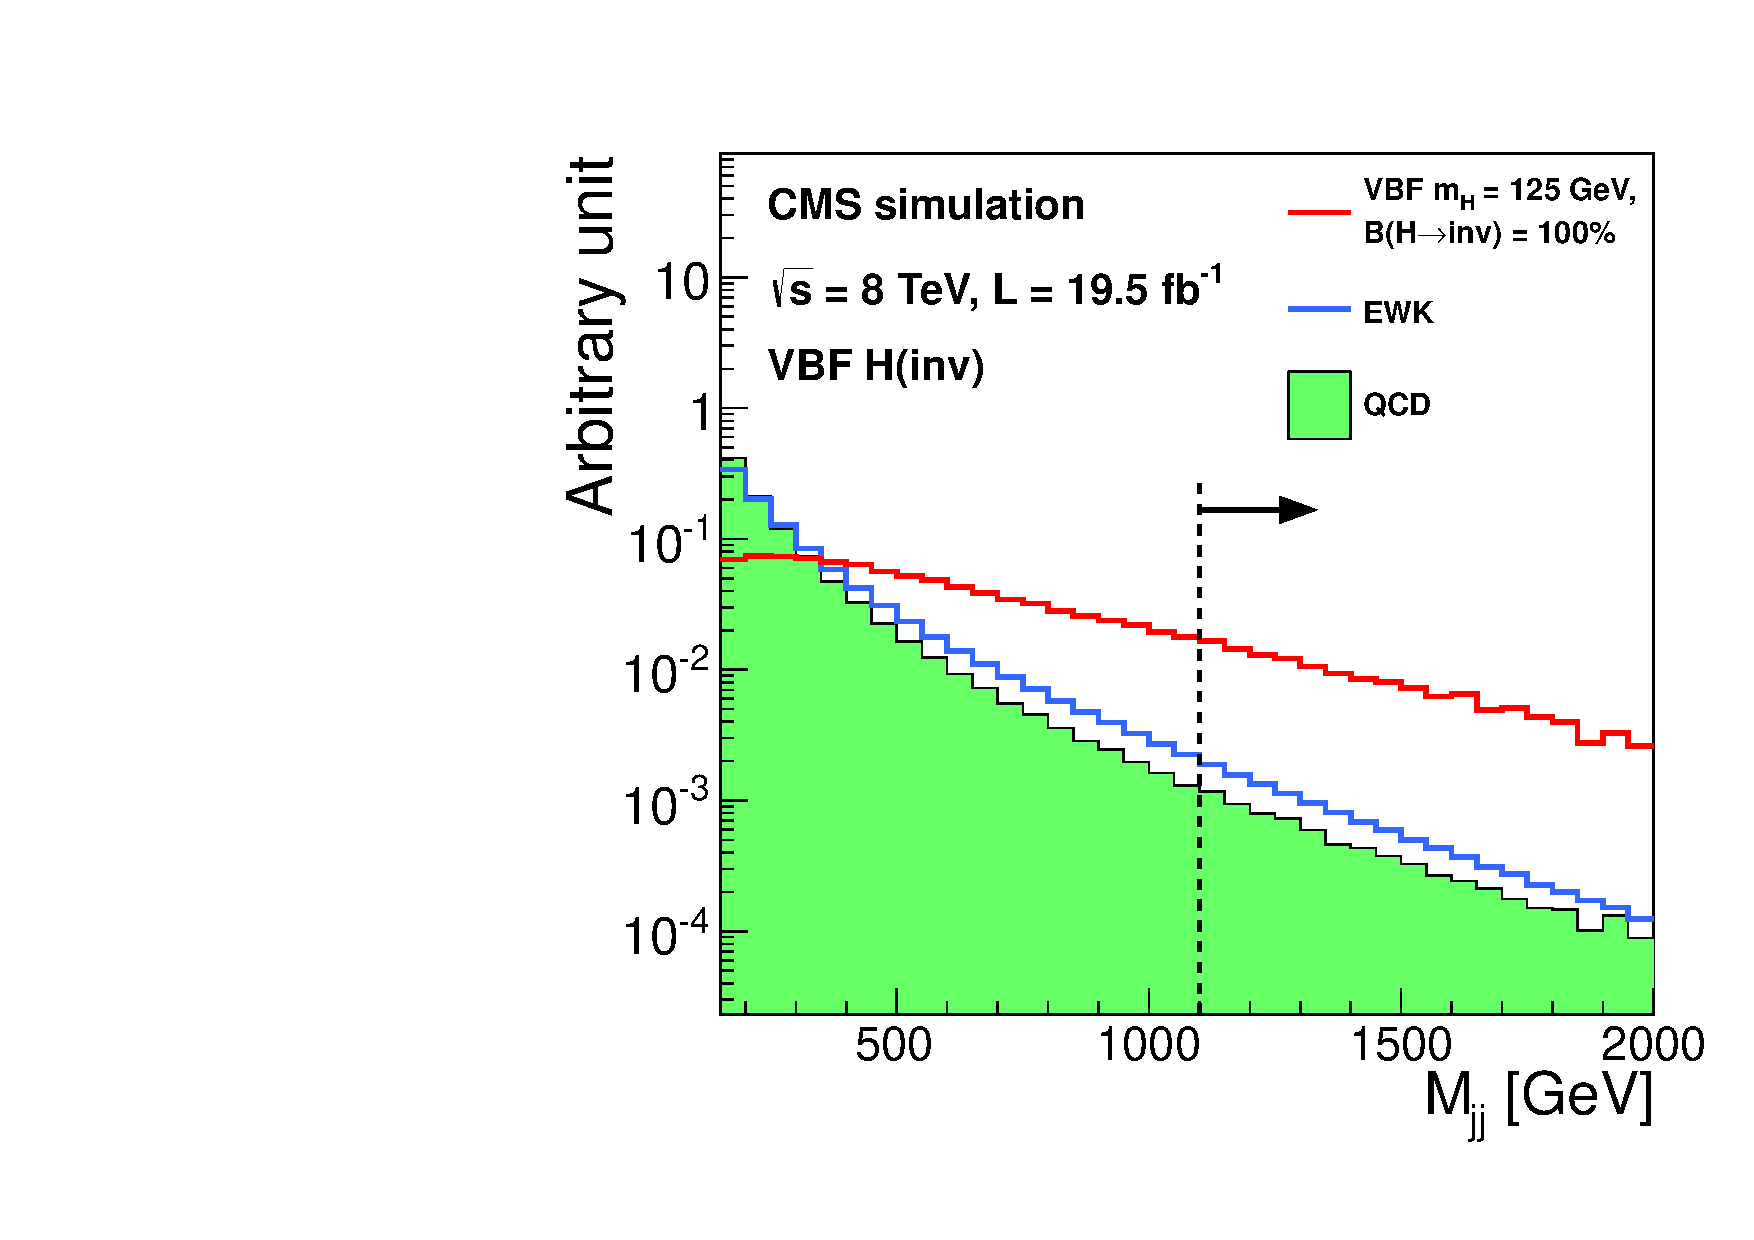
\includegraphics[width=.6\largefigwidth]{plots/prompt/VBF-Dijet-M.pdf}}
  \subfloat[]{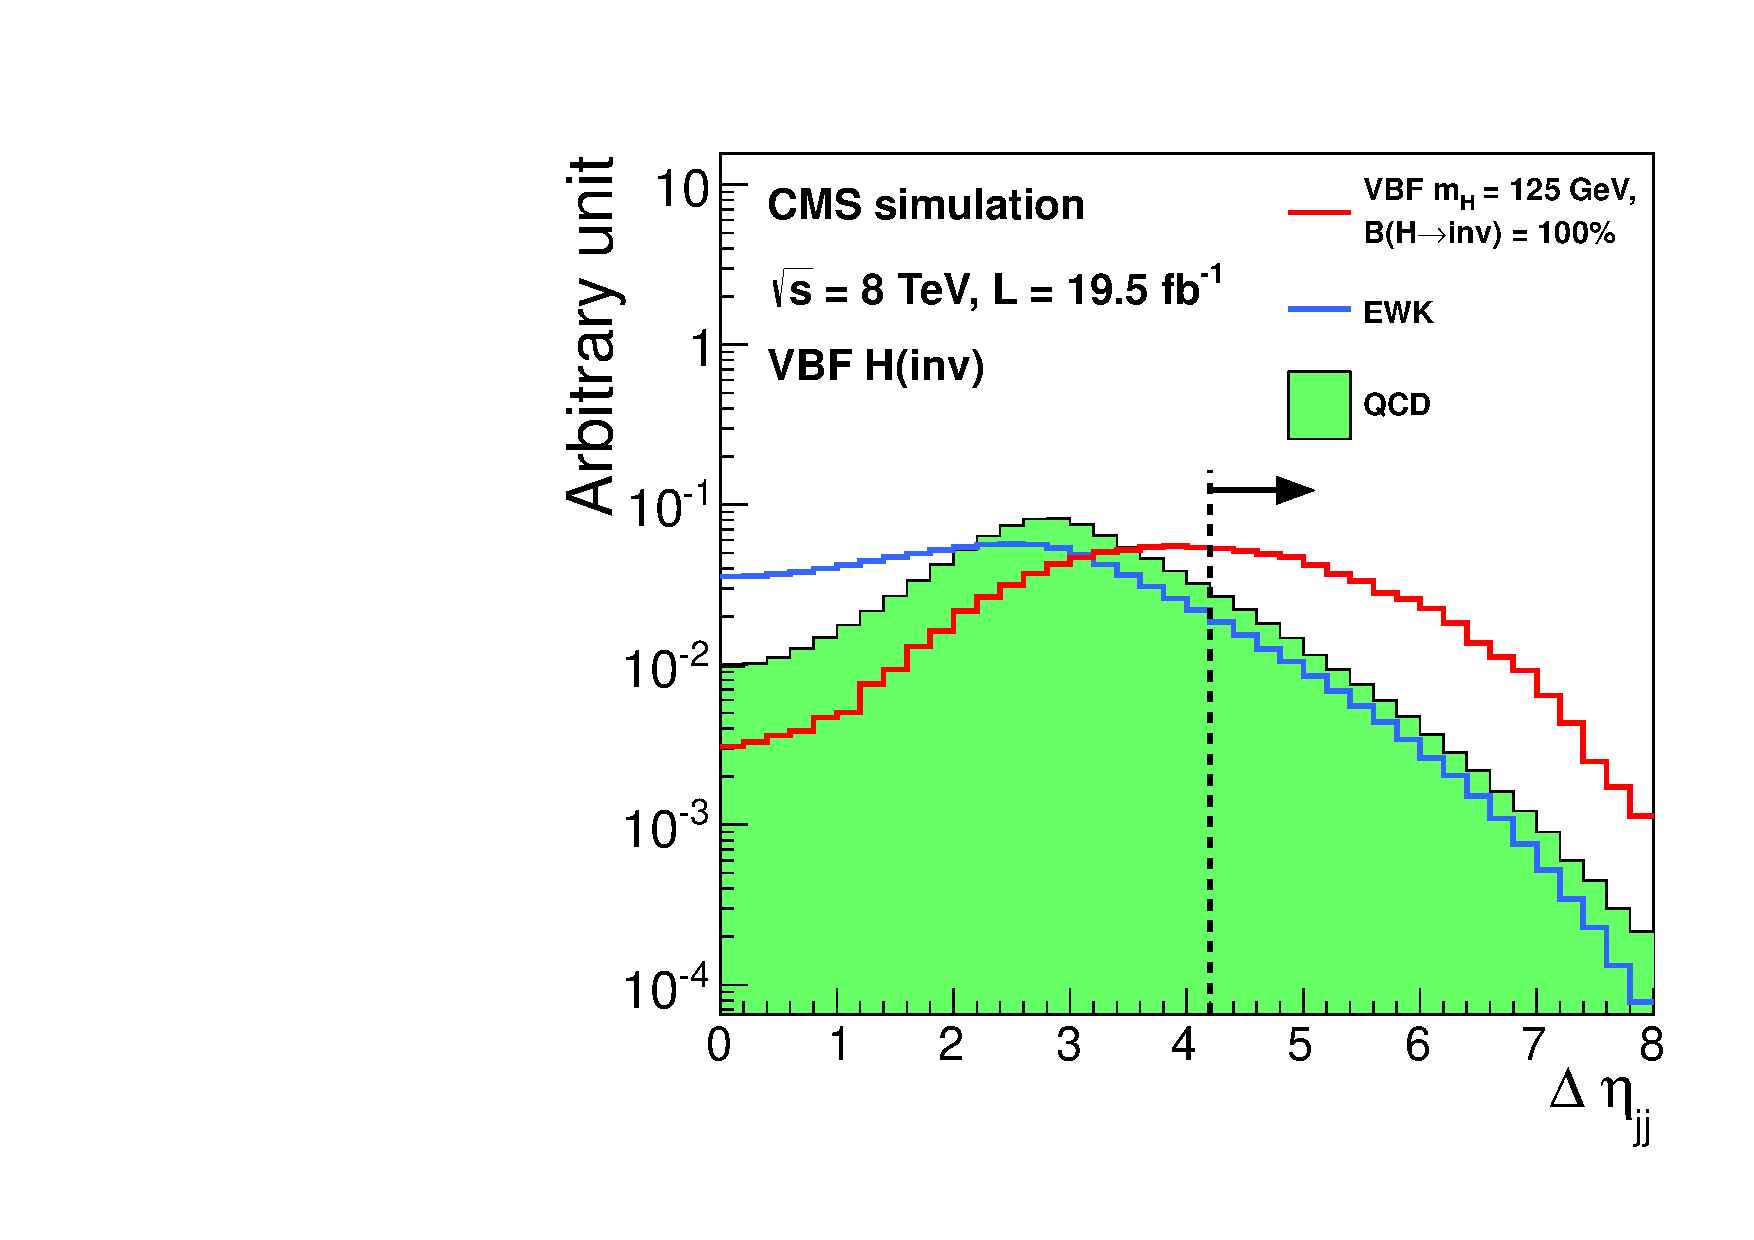
\includegraphics[width=.6\largefigwidth]{plots/prompt/VBF-Dijet-DEta.pdf}}

  \subfloat[]{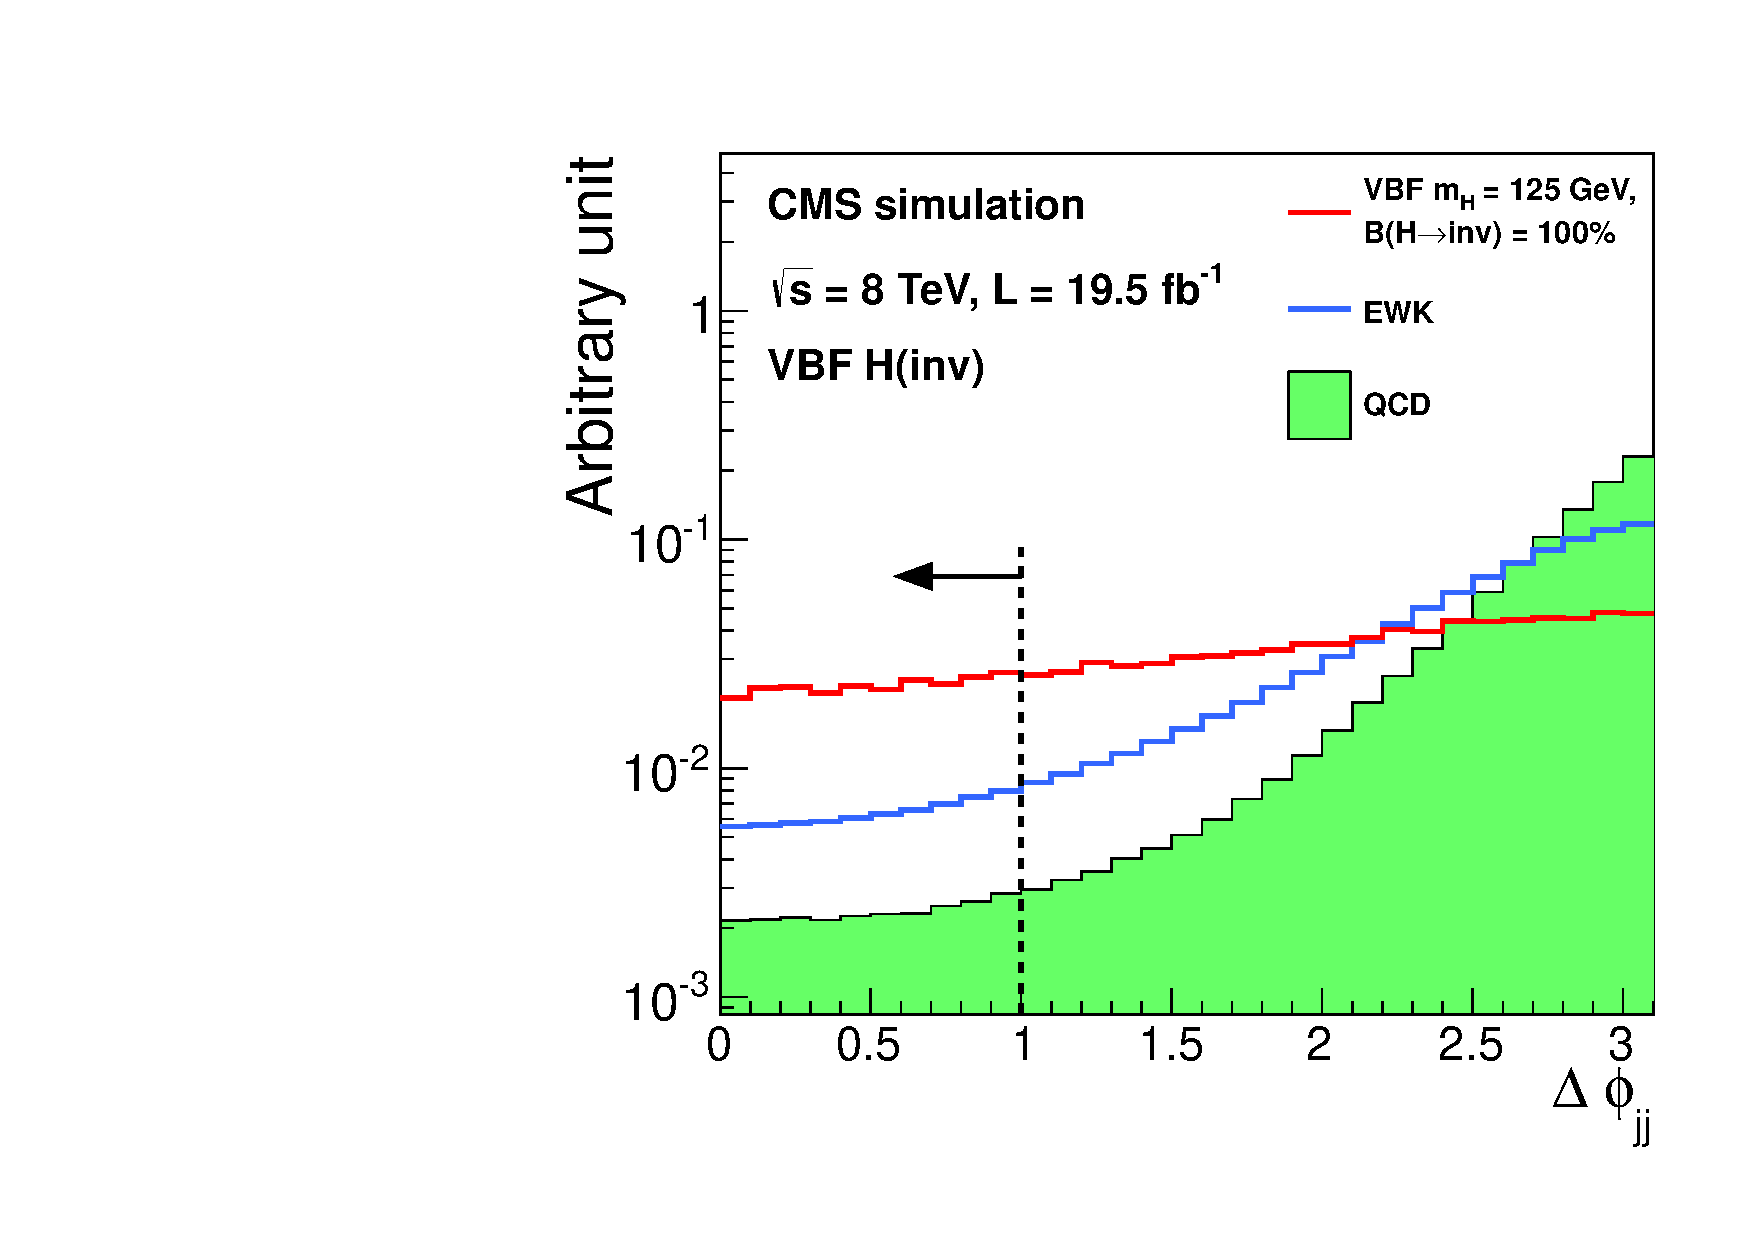
\includegraphics[width=.6\largefigwidth]{plots/prompt/VBF-Dijet-DPhi.pdf}}
  \subfloat[]{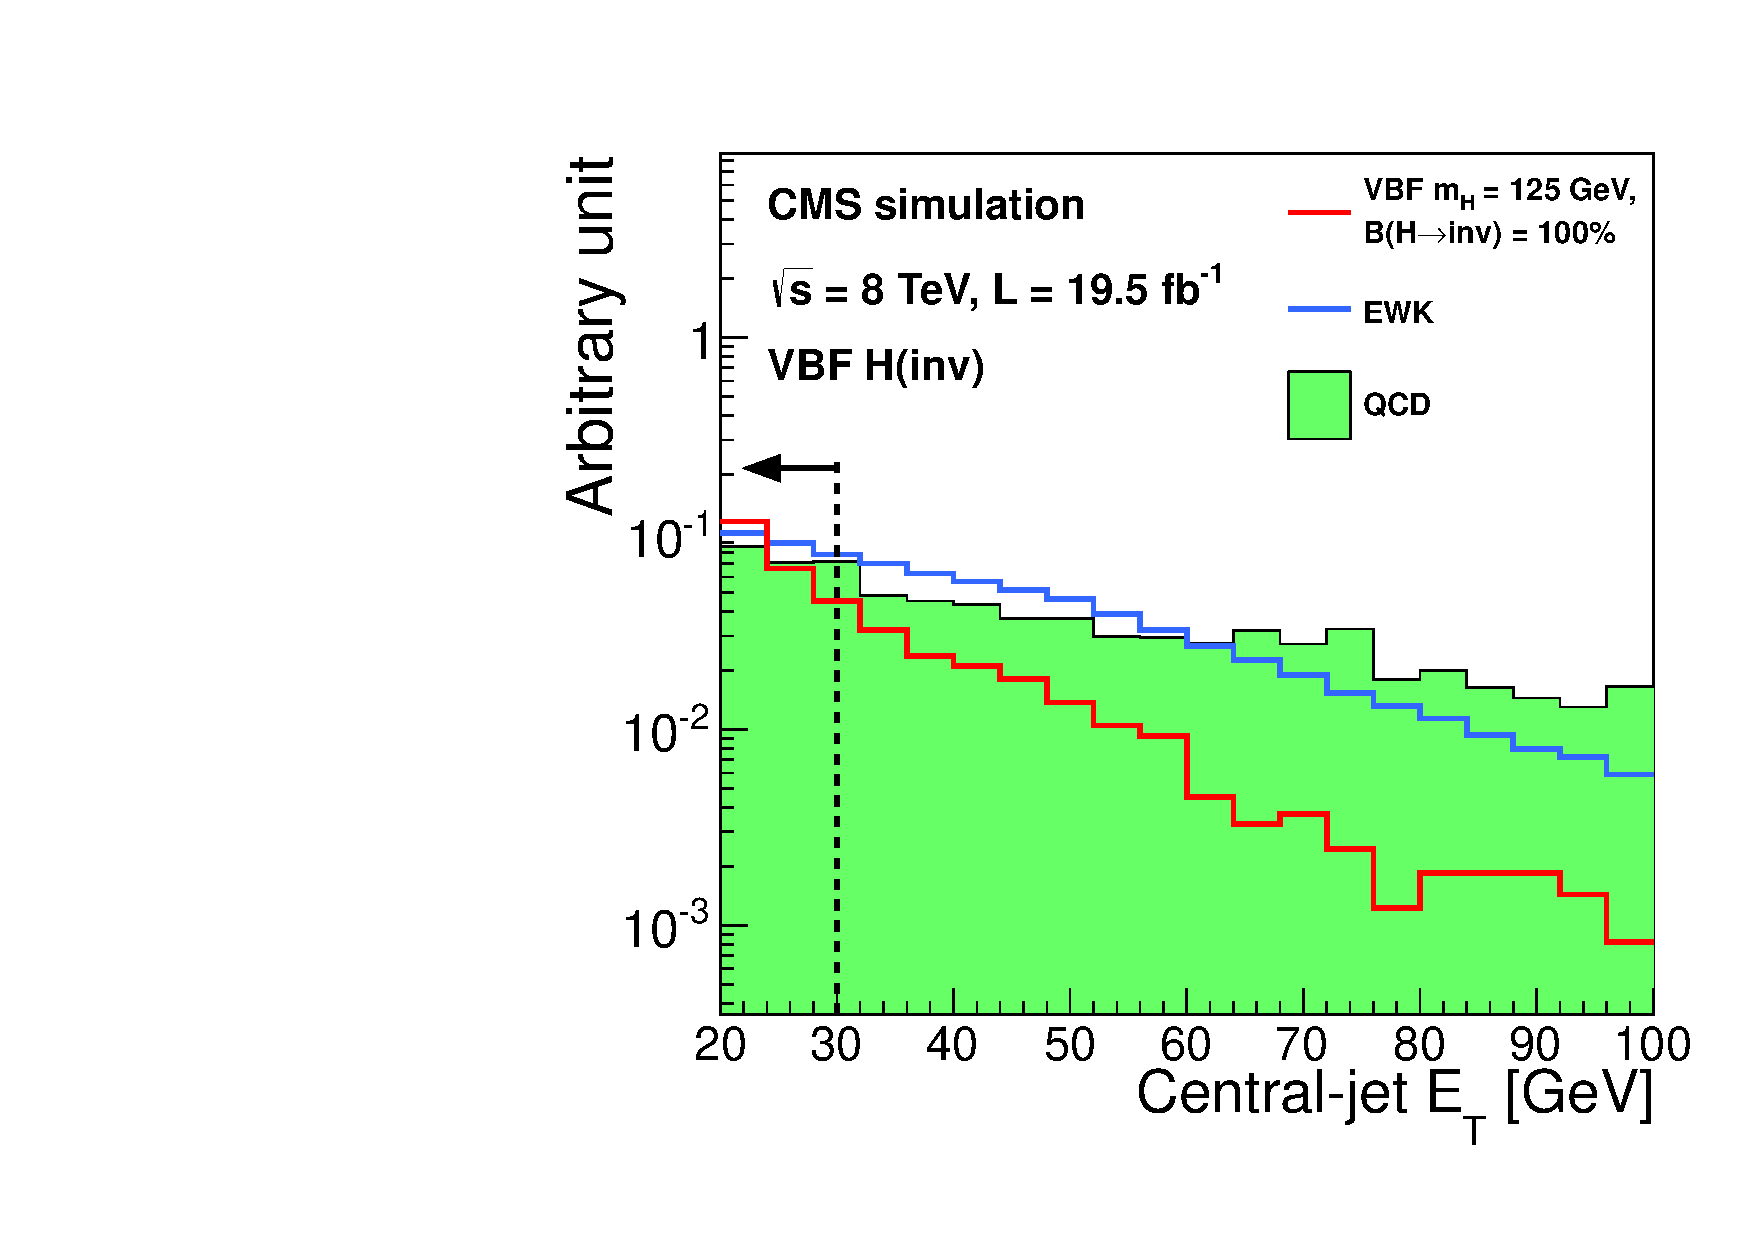
\includegraphics[width=.6\largefigwidth]{plots/prompt/VBF-CJV-pT.pdf}}
  \caption{Distributions of (a) $M_{jj}$, (b) $\Delta\eta_{jj}$, (c) $\Delta\phi_{jj}$ and (d) leading central jet \pt in background and signal \ac{MC} events. The events shown are required to have two jets in opposite forward/backward halves of the detector with \pt$>50$ \GeV, $|\eta|<4.7$, $M_{jj}>150$ \GeV and \MET$>130$ \GeV. The dashed lines indicate the offline selection criteria applied to these variables ~\cite{Chatrchyan:2014tja}.}
  \label{fig:promptcontrolplots}
\end{figure}


\section{Background estimation}%??
\label{sec:promptbkg}
As discussed in \SectionRef{sec:promptsel} there are several background processes which are capable of producing VBF-like jets in association with \MET. The analysis' event selection removes most of the events from these processes, however a significant number still remain and it is important to estimate this number precisely. Data-driven methods, where data ``control regions'', which are similar to the signal region, are used to estimate the most significant backgrounds. This data-driven approach is particularly important due to the very stringent kinematic requirements placed on the tag jets, which lead to high uncertainties on estimates taken from \ac{MC} alone. The particular method used to estimate each of the backgrounds will be described in this section.

\subsection{\PW$\rightarrow e\nu$ + jets}%??
\label{sec:promptwenu}
The background from the production of a $\PW$ boson in association with jets, ``$\PW$+jets'' where the $\PW$ boson decays to an electron and an electron neutrino, $\PW\rightarrow e\nu$ is estimated using single electron events. All aspects of the event selection are the same as those used in the singal region, except for the electron veto, which is replaced with the requirement that there is exactly one tight electron, with $p_{T}>20$ \GeV, in the event and no other veto electrons. These requirements give a single electron control region with events with jets that have the same kinematics as those in the signal region, but which is dominated by $\PW$ boson decays to electrons.

The estimated number of $\PW\rightarrow e\nu$ events in the signal region is then estimated by using the ratio between the expected number of events in the signal and control regions from \ac{MC} to extrapolate from the number of events seen in data in the single electron control region using the following formula:
\begin{equation}
  \label{eq:wdatabkg}
  N^{S}_{Exp}=\left(N^{C}_{Data}-N^{C}_{Bkg}\right)\cdot\frac{N^{S}_{MC}}{N^{C}_{MC}},
\end{equation}
where $N^{S}_{Exp}$ is the number of expected events in the signal region from this background process, $N^{C}_{Data}$ is the number of events seen in the control region in data, $N^{C}_{Bkg}$ is the number of events from other backgrounds in the control region estimated using \ac{MC}, which is expected to be small, and $N^{S}_{MC}$ and $N^{C}_{MC}$ are the numbers of events predicted by \ac{MC} to be in the signal and control regions respectively. The fact that estimations from \ac{MC} are only used in ratios or where they are expected to be small removes any dependence of the final background estimation on the overall rate of the process predicted by \ac{MC}, and instead allows the observed rate in data to be used.

%??plot or table

\subsection{\PW$\rightarrow \mu\nu$ + jets}%??
\label{sec:promptwmunu}
The method used to estimate the background from $\PW$+jets where the $\PW$ boson decays to a muon and a muon neutrino, $\PW\rightarrow\mu\nu$, is very similar to that used for $\PW\rightarrow e\nu$. A single muon control region is used, again with identical selection to the signal region except for the modification of the lepton veto, in this case by replacing the muon veto with the requirement that there is exactly one tight muon, with \pt$>20$ \GeV, and no other veto muons. \EquationRef{eq:wdatabkg} is then used, with the control region now being the single muon control region, to estimate the number of events from $W\rightarrow\mu\nu$ expected in the signal region.

%??plot or table

\subsection{\PW$\rightarrow \tau\nu$ + jets}%??
\label{sec:promptwtaunu}
The background from $\PW$+jets where the $\PW$ boson decays to a tau and a tau neutrino, $\PW\rightarrow\tau\nu$, is estimated using a single tau control region data-driven method. However, in this case the control region used has more differences from the signal region than those used above. The reason for these increased differences is that the reconstruction efficiency for tau leptons is significantly lower than that for electrons or muons, and they are also more likely to be misreconstructed as jets, causing the event to be vetoed by the \ac{CJV}. The single tau control region has the same requirements as the signal region except that the \ac{CJV} is removed and exactly one tau with \pt$>20$ \GeV\, is required.
%??same again, but stats (exactly how many mean has to be looser (NO CJV), overlap issue with signal region which is small due to looser region and low stats, cross-check of tau discriminant

%??plot or table

\subsection{\PZ$\rightarrow \nu\nu$ + jets}%??
\label{sec:promptznunu}

%??new formula and reason, region including Z mass constraint, MC sample switcheroo

%??plot or table/both

\subsection{QCD}%??
\label{sec:promptQCD}
%??ABCD method, others that were tried and why went for ABCD

\subsection{Minor backgrounds}%??
\label{sec:promptminor}
%??from MC, doesn't matter because they're small

\section{Systematic uncertainties}%??
\label{sec:promptsyst}
%??Systematics

\section{Results}%??
\label{sec:promptresults}
